\chapter{Аналитический раздел}

В данном разделе проводится обзор существующих способов описания трехмерных моделей, алгоритмов построения трехмерного изображения. Осуществляется анализ существующих моделей освещения и алгоритмов закраски полигонов.

\section{Описание сцены}

В компьютерной графике сцена является неотъемлемым компонентом, содержащим в себе всю информацию, необходимую для синтеза изображения. Поэтому определение ее структуры является одним из важнейших и первостепенных шагов в создании программы.

Сцена будет представлена структурой, содержащей в себе коллекцию из объектов и коллекцию из источников освещения. Размеры этих коллекций будут ограничены лишь объемом оперативной памяти.

\section{Описание моделей трехмерных объектов в сцене}

Существует множество способов представления трехмерных объектов в сцене. Различным алгоритмам отрисовки требуется разная информация о самом объекте.

\subsection{Функциональное моделирование}

Одним из простейших способов задания трехмерных объектов можно назвать функциональное моделирование. Возможны несколько вариантов:

\begin{enumerate}
	\item Поверхность такого объекта задается системой уравнений

	\begin{equation}
		\left\{
		\begin{array}{l}
			x = x(u, v) \\
			y = y(u, v) \\
			z = z(u, v) \\
		\end{array}
		\right.,
	\end{equation}
	
	В этом случае каждая точка на поверхности объекта из плоской системы координат $(u, v)$ преобразуется в мировое пространство $(x, y, z)$.

	\item Внутренний объем такого объекта выражается неравенством:
	
	\begin{equation}
		f(x, y, z) > 0.
	\end{equation}

	Данное неравенство справедливо для всех точек внутри объекта.
\end{enumerate}

Особенности данного представления:

\begin{itemize}[$\bullet$]
	\item Функциональное моделирование позволяет получить максимальный уровень детализации при отрисовке, наилучшую сглаженность формы объекта.
	\item Достаточно сложная форма может иметь довольно простое параметрическое представление, из чего следует меньший расход памяти при хранении представления объекта.
	\item Трансформации над объектом производятся очень просто. Достаточно применить преобразования к описывающим объект уравнениям или неравенствам.
	\item Наложение текстур в случае с внутренне-определёнными объектами является затруднительным.
	\item Процесс отыскания параметрического представления невыпуклых многогранников может быть затруднительным.
\end{itemize}

\subsection{Полигональная сетка}

Другим представлением трехмерных объектов в сцене является представление в виде полигональной сетки -- совокупностью вершин, ребер и граней, которые определяют форму объекта \cite{net-model}.

 Структура полигональной модели представлена на рисунке \ref{pic:net}.

$\backslash$ тут картинка (Рисунок 1.1 - Структура полигональной модели)

\begin{figure}
	\centering
	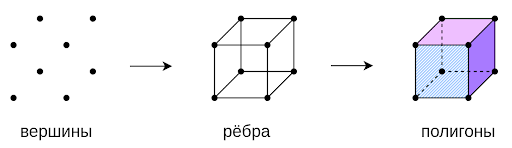
\includegraphics[width=0.6\linewidth]{pic:net.png}
	\caption{Структура полигональной модели}
	\label{pic:net}
\end{figure}

Полигональная сетка состоит из набора отдельных полигонов, которые в свою очередь являются многоугольниками, ребра которых соединяют вершины сетки [1]. Полигональная сетка является аппроксимацией поверхности представляемого объекта. От её плотности, т.е. от количества полигонов на единицу объема, зависит качество изображения объекта.

Так как полигоны в сети могут представляться вне зависимости друг от друга, данный способ позволяет с меньшей сложностью описать объекты нетривиальной формы в сцене. Перечислим особенности данного представления:

\begin{itemize}[$\bullet$]
	\item Просто создать топологию поверхности.
	\item Преобразования над объектом сводятся к преобразованию полигональной сетки, что в свою очередь раскладывается на независимые преобразования над отдельными полигонами.
	\item Наложение текстур на поверхность является несложной процедурой.
	\item Повышение плотности сетки приводит к увеличению объема затрачиваемой памяти для ее хранения.
\end{itemize}

\subsection{Воксельная сетка}

Наконец, есть еще один способ представления трёхмерных объектов - представление воксельной сеткой. Объем - это трехмерный массив кубических элементов (вокселей), представляющих единицы 3D пространства [2]. Воксельная сетка позволяет непосредственно представить объем объекта, его внутреннее содержание. Выделим особенности данного представления:

\begin{itemize}
	\item Просто представляются объекты сцены.
	\item Легко выполняются отсечения частей объекта. Достаточно сделать часть вокселей прозрачными.
	\item Текстурирование тесно связано с воксельной сеткой. Нельзя изменить текстуру объекта без изменения воксельной сетки.
	\item Поворот и масштабирование объекта не могут быть осуществлены без перерасчета сетки.
	\item Чем больше объем объекта, тем больше затрачивается памяти на хранение его представления.
\end{itemize}

\subsection{Вывод}

Для решения поставленных задач лучше всего подходит метод с использованием полигональной сетки для представления поверхностей объектов, так как он рассчитан на широкий круг задач моделирования, позволяет легко модифицировать положение объекта в пространстве, а также прост в реализации.

\section{Алгоритмы построения трехмерного изображения}

Проведем сравнительный анализ алгоритмов построения трехмерного изображения для выбора наиболее подходящего. Целевыми показателями, на которые следует обратить внимание являются: зависимость скорости работы от числа изображаемых объектов на сцене, требуемый объем памяти, а также возможность распараллеливания процесса работы алгоритма.

\subsection{Алгоритм художника}

Принцип данного алгоритма заключается в том, что объекты на экране рисуются в порядке от дальних к ближним, при этом происходит наложение - ближние объекты рисуются поверх дальних. Этот алгоритм удобен в случаях, когда процесс распознавания видимых частей объекта является более затратным, чем собственно его полная отрисовка. Но при этом этот алгоритм производит лишнюю работу по отрисовке невидимых частей объектов.

\subsection{Алгоритм Вейлера-Азертона}

Алгоритм Вейлера-Азертона позволяет выполнить отсечение невидимой части объекта перед его отрисовкой по контурам загораживающих его объектов. Этот прием позволяет не делать лишнюю работу при отрисовке частично видимых объектов. На рисунке 1.3 показано разбиение многоугольников.

$\backslash$ picture (Рисунок 1.3 - Разбиение многоугольников по алгоритму Вейлера-Азертона)

\subsection{Алгоритм с использованием Z-буфера}

Алгоритм с использованием Z-буфера базируется на том, что вместо того, чтобы определять очередность в которой должны отрисовываться объекты, для каждого пикселя при отрисовке сохраняется дополнительный атрибут - глубина, использование которого гарантирует корректное отображение пикселя, соответствующего наиболее близкому объекту.

\subsection{Алгоритм обратной трассировки лучей}

Алгоритм обратной трассировки лучей базируется на физическом представлении света и законах геометрической оптики. Он позволяет с высокой степенью точности моделировать различные оптические эффекты.

\subsection{Вывод}

Для программной реализации отображения сцены на экран было решено выбрать алгоритм трассировки лучей как основной для создания реалистического изображения, а при временной отрисовке использовать алгоритм Z-буфера.

\section{Методы закраски}

При использовании алгоритмов, основанных на закрашивании полигонов, следует подобрать модель освещения в сцене, т.к. это напрямую влияет на изменение цвета в пределах одного полигона.

\subsection{Простая закраска}

При реализации простой закраски для каждой отдельно взятой грани объекта используется информация об источниках света для расчета цвета, в который впоследствии закрашивается эта грань. Простая закраска хорошо подходит для граненых объектов, которым не требуется сглаживание.

\subsection{Закраска по Гуро}

Закраска по Гуро учитывает кривизну поверхности и использует бикубическую интерполяцию для расчета цвета очередного пикселя. Интерполируемым значением является цвет граничных пикселей. Данный вид закраски позволяет с достаточной степенью точности изображать гладкие кривые поверхности [4].

\subsection{Закраска по Фонгу}

Закраска по Фонгу также учитывает искривленные поверхности, но за счёт интерполяции не цвета пикселя, а вектора нормали, для которого и происходит перерасчет значения интенсивности цвета пикселя. Такой метод позволяет гораздо точнее учитывать блики на поверхности объектов, а также позволяет корректно обрабатывать случаи, когда источник света расположен вблизи освещаемого объекта [4].

\subsection{Метод освещения}

Для реализации освещения в сцене будет использоваться глобальная модель освещенности, а для создания теней - алгоритм трассировки лучей от поверхности отображаемого полигона до всех источников освещения.

\subsection{Вывод}

Для закраски полигонов было решено реализовать все три метода и предоставить пользователю  возможность изменять метод закраски в процессе работы программы. Простой метод закраски может быть использован для быстрого, но менее реалистичного синтеза изображения, в то время как с помощью остальных методов закраски изображение синтезируется значительно медленнее, но имеет более реалистичный вид.

\chapter{Конструкторский раздел}

Данный раздел посвящен конструированию приложения, а также описанию алгоритмов и методов, которые будут применяться в разрабатываемой программе.

\section{Требования к программе}

Создаваемая программа должна предоставлять следующий набор функций:

\begin{itemize}[$\bullet$]
	\item Загрузка заготовленных полигональных моделей из файлов.
	\item Добавление в сцену объектов из заготовленного набора примитивов.
	\item Независимое трансформирование положения объектов в сцене.
	\item Навигация по сцене с помощью перемещения и поворота главной камеры.
	\item Просмотр и изменение специфических свойств объектов в сцене.
	\item Сохранение текущего изображения сцены в файл на диске.
	\item Сохранение созданной сцены в файл на диске.
	\item Загрузка готовой сцены из файла.
\end{itemize}

\section{Описание основных алгоритмов}

В данном подразделе будут приведены описания используемых алгоритмов с представлением соответствующих схем алгоритмов.

\subsection{Алгоритм визуализации трехмерной сцены с использованием Z-буфера}

\subsection{Алгоритм отображения части полигона в буфер}

\subsection{Алгоритм обратной трассировки лучей}

\section{Выбор используемых типов и структур данных}

Математические абстракции:

\begin{itemize}
	\item Четырехкомпонентный вектор
	\item Матрица 4х4
	\item Луч. Состоит из двух векторов - начала и направления
	\item Прямоугольная двухмерная область
\end{itemize}

Примитивы растеризации:

\begin{itemize}
	\item Пиксель (в формате ARGB32)
	\item Цель отрисовки. Содержит буфер из пикселей, в который происходит отрисовка, и размеры окна - ширина и высота.
\end{itemize}

Сцена и объекты сцены:

\begin{itemize}
	\item Вершина полигона. Состоит из позиции и вектора нормали.
	\item Полигон. Состоит из трех вершин полигона.
	\item Полигональная модель. Состоит из массива полигонов.
	\item Источник света. Содержит тип (точечный/направленный), вектор положения/направления, интенсивность и цвет.
	\item Камера. Содержит матрицу проецирования на экранную плоскость.
	\item Сцена из объектов. Состоит из списка полигональных моделей и списка источников света.
\end{itemize}

\chapter{Технологический раздел}

Данный раздел посвящен выбору средств для программной реализации разработанного метода, описанию основных моментов разработки программного обеспечения.

\section{Выбор языка программирования и среды разработки}

Для написания программы в качестве языка программирования был выбран язык С++ по следующим причинам:

\begin{itemize}
	\item Имеет статическую типизацию, является компилируемым языком программирования;
	\item Позволяет напрямую работать с памятью, а также контролировать все обращения к менеджеру памяти;
	\item Имеет мощный механизм шаблонов;
	\item Позволяет писать программы как в структурном стиле, так и в объектно-ориентированном;
\end{itemize}

В качестве среды разработки была выбрана <<CLion>> по следующим причинам:

\begin{itemize}
	\item Кроссплатформенность среды и разрабатываемого ПО;
	\item Данная среда разработки использует утилиту CMake для сборки проектов;
\end{itemize}

\section{Схема доменов}

Программа состоит из трех доменов: прикладного, архитектурного и интерфейсного. Прикладной домен отвечает за процесс визуализации сцены, интерфейсный - за взаимодействие с пользователем, а архитектурный служит связующим звеном между двумя вышеупомянутыми доменами.

\section{Прикладной домен}

Прикладной домен реализуется в структурном стиле, так как такой подход обеспечивает наибольшую скорость работы и простоту реализации, а также в дальнейшем не нуждается в частых модификациях.

\section{Архитектурный домен}

Архитектурный домен реализуется согласно объектно-ориентированному подходу с использованием паттернов проектирования. Информационная модель архитектурного домена представлена на рисунке 3.4.

\section{Интерфейсный домен}

Интерфейсный домен реализуется с использованием открытой библиотеки Qt. Результат разработки программного обеспечения представлен в приложении А.

\chapter{Экспериментальный раздел}
